Korzystając z~wiedzy i~doświadczeń wyniesionych z~sekcji~\ref{sec:przeglad} niniejszego sprawozdania, zdecydowaliśmy się na stworzenie systemu odpowiadającego na pytania ogólne, z~wyszczególnieniem pytań o~fakty dotyczące:
\begin{itemize}
	\item osób,
	\item miejsc,
	\item dat,
	\item cech wielkościowych,
	\item przedmiotów.
\end{itemize}

Bazą wiedzy systemu jest sieć WWW. Do wyszukiwania dokumentów w~sieci~WWW, wykorzystane zostały wyszukiwarki internetowe: \emph{Google\footnote{www.google.pl}}, \emph{Bing\footnote{www.bing.com}}, \emph{Yahoo\footnote{www.search.yahoo.com}} oraz \emph{DuckDuckGo\footnote{duckduckgo.com}}. Dodatkowo wprowadzona została opcja \emph{combined}, która zwraca rezultaty uzyskane ze wszystkich wymienionych wyżej stron. Zapytanie do wyszukiwarki jest tworzone za pomocą jednej z trzech strategii: \emph{singleQuery}, \emph{stopwords} lub \emph{chunks}. Pierwsza polega na bezpośrednim wyszukaniu wpisanego pytania, druga usuwa wyrazy ze Stop-listy przed rozpoczęciem wyszukiwania, ostatnia tworzy wiele zapytań poprzez podział zapytania na kawałki, tzw. \emph{chunks}. 

Podobnie jak we wcześniej omawianym systemie AskMSR~\cite{brill2002analysis}, do dalszej analizy przekazywane są jedynie \emph{snippety}, co pozwoliło na uproszczenie etapu filtracji akapitów. 

Odpowiedzią na przedstawione pytanie, jest prosta jedno-, dwu- lub trzywyrazowa odpowiedź typu \emph{Named-Entity} oraz adres URL, z której pochodzi dany \emph{snippet}. 

\subsection{Opis algorytmu}
Na rysunku~\ref{fig:algorithm-overview}, przedstawiony został ogólny schemat algorytmu odpowiadania na pytania.

\begin{figure}[h]
    \centering
    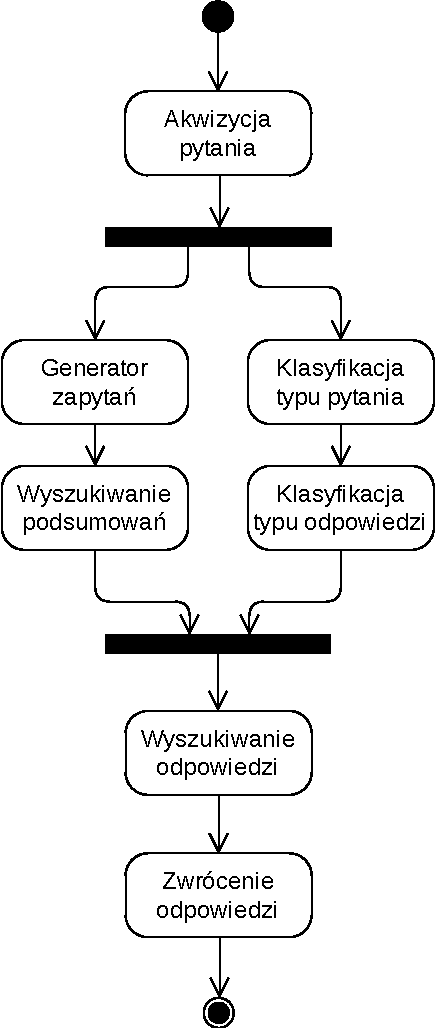
\includegraphics[width=0.7\columnwidth]{figures/WEDT-Algorytm.pdf}
    \caption{Ogólny schemat algorytmu odpowiadania na pytania}
    \label{fig:algorithm-overview}
\end{figure}

\subsubsection{Akwizycja pytania}
Pierwszym krokiem algorytmu jest akwizycja pytania od użytkownika systemu. Każde pytanie jest analizowane w~sposób indywidualny, bez przechowywania wcześniejszych pytań i~utrzymywania kontekstu. Nie zakładamy również żadnego profilowania użytkowników, ponieważ typowo proste pytania o~fakty, są ze sobą słabo powiązane. Dla każdego zapytania użytkownik wybiera strategię wyszukiwania tj. \emph{singleQuery}, \emph{stopwords} lub \emph{chunks} oraz jedną z 5 opcji wyszukiwania: \emph{Google}, \emph{Bing}, \emph{Yahoo}, \emph{DuckDuckGo} lub \emph{combined}.

\subsubsection{Klasyfikacja typu pytania}
W~kolejnym kroku następuje klasyfikacja typu pytania, a zaraz po niej określenie typu oczekiwanej odpowiedzi. Klasy pytań są definiowane przez zaimki pytające, podobnie jak w~\cite{gupta2012survey}. W naszym systemie wyróżniamy 16 rodzajów pytań. Rozpoznawane są zarówno formy podstawowe zaimków pytających, jak i formy odmienione.

Klasyfikacja typu pytania jest ściśle powiązana z pierwszym z dwóch etapów rozpoznawania typu odpowiedzi. Aby wykryć typ pytania, słowa z zapytania są kolejno sprawdzane w przygotowanym słowniku zawierającym pary typPytania-typOdpowiedzi, gdzie typPytania jest kluczem, natomiast typOdpowiedzi wartością. Słowo z zapytania, które jako pierwsze będzie miało przyporządkowaną wartość w słowniku, informuje o typie pytania. Od tej reguły istnieje jeden wyjątek, który wymusza sprawdzenie również kolejnych wyrazów z zapytania. Przy pytaniach \emph{Co ile ... ?}, typ pytania jest określony przez drugi wyraz z zapytania posiadający odpowiednik w słowniku. Rozpoznawane pary typPytania-typOdpowiedzi przedstawiono w tabeli~\ref{tab:tabelaPytOdp}.

\begin{table}[h]
	\centering
	\begin{tabular}{|c|c| }
		
		 \hline
		\textbf{typPytania} & \textbf{typOdpowiedzi}  \\ \hline
		czyj? & OSOBA \\  \hline
		komu? & OSOBA \\ \hline
		kogo? & OSOBA \\ \hline
		kim? & OSOBA \\ \hline
		kiedy? & DATA \\  \hline
		ile? & WIELKOŚĆ \\  \hline
		co? & RZECZ \\  \hline
		czego? & RZECZ \\ \hline
		czym? & RZECZ \\ \hline
		skąd? & MIEJSCE \\ \hline
		dokąd? & MIEJSCE \\ \hline
		gdzie & MIEJSCE, RZECZ \\ \hline
		kto & OSOBA, MIEJSCE \\ \hline
		jak & complex \\ \hline
		który? & complex \\ \hline
		jaki? & complex  \\  \hline
	\end{tabular}
	\caption{Rozpoznawane pary typPytania-typOdpowiedzi}

\label{tab:tabelaPytOdp}

\end{table}

\subsubsection{Klasyfikacja typu oczekiwanej odpowiedzi}
Rozpoznawanie typu odpowiedzi składa się z jednego lub dwóch etapów. Etap pierwszy odbywa się równocześnie z rozpoznawaniem typu pytania, ponieważ zwracana wartość ze słownika to typ oczekiwanej odpowiedzi. Pojedyncze rozpoznawane typy to: OSOBA, MIEJSCE, RZECZ, WIELKOŚĆ oraz DATA. Danemu typowi pytania może być przyporządkowana jeden lub więcej typów oczekiwanej odpowiedzi. Nie wszystkie typy pytań jednoznacznie określają oczekiwany typ odpowiedzi, dlatego dla niektórych pytań niezbędne okazało się wprowadzenie drugiego etapu. Pytania \emph{Jak?}, \emph{Jaki/Jaka/Jakie?}, oraz \emph{Który/Która/Które?} są nietrywialne, ponieważ nie można jednoznacznie przyporządkować typu oczekiwanej odpowiedzi (\emph{complex}) bez dodatkowej analizy zapytania. 

Przy pytaniach \emph{Jaki/Jaka/Jakie?} oraz \emph{Który/Która/Które?} pierwszy krok do odnalezienia typu odpowiedzi polega na sprawdzeniu czy pomiędzy zaimkiem pytającym a czasownikiem, występuje rzeczownik, którego odmiana tj. liczba oraz przypadek, zgodna jest z odmianą zaimka pytającego. W tym celu wykorzystane zostało narzędzie \emph{Spejd}, które zwraca między innymi leksemy poszczególnych wyrazów jak i tagsety zawierające informacje o częściach mowy i ich odmianie. Leksem odpowiednio odmienionego rzeczownika jest następnie analizowany za pomocą narzędzia \emph{plWordNet}. Zwraca ono między innymi listę domen, do których przynależy dany rzeczownik. Domeny z \emph{plWordNetu} konwertowane są na jedną lub więcej oczekiwanych typów odpowiedzi z listy: OSOBA, MIEJSCE, RZECZ, WIELKOŚĆ, DATA lub brak dopasowania. Jeżeli do danego rzeczownika nie zostanie przyporządkowana żadna domena z listy, zapytanie nie zostanie dalej przetworzone. Jeżeli natomiast pomiędzy zaimkiem pytającym a czasownikiem nie występuje żaden pasujący rzeczownik, algorytm próbuje odnaleźć poprawnie odmieniony przymiotnik znajdujący się pomiędzy zaimkiem a czasownikiem. Gdy takowy występuje, oczekiwanym typem odpowiedzi jest WIELKOŚĆ. 
Jeżeli taki przymiotnik nie zostanie odnaleziony, ostatnią szansą jest odszukanie rzeczownika w pozostałej części zapytania tj. za czasownikiem. Odmiana rzeczownika również musi być zgodna z odmianą zaimka pytającego. Jeżeli zostanie on odnaleziony, to dalsze postępowanie jest analogiczne do sytuacji z rzeczownikiem znajdującym się pomiędzy zaimkiem a czasownikiem. Dodatkowo wyszczególniony został przypadek pytań w stylu \emph{Który z?}. Dla takiego przypadku poszukiwany jest rzeczownik w liczbie mnogiej w dopełniaczu znajdujący się pomiędzy zaimkiem pytającym a czasownikiem.

Przy pytaniu \emph{Jak?} najpierw poszukiwany jest przymiotnik znajdujący się pomiędzy zaimkiem pytającym a czasownikiem. Jeżeli taki zostanie odnaleziony, szukanym typem odpowiedzi jest WIELKOŚĆ. W przeciwnym wypadku oczekiwanym typem może być zarówno WIELKOŚĆ, OSOBA, MIEJSCE czy RZECZ. 

\subsubsection{Generator zapytań}
Generator zapytań otrzymuje pytanie wprowadzone przez użytkownika wraz ze strategią generowania zapytania. Jeżeli wybrana została strategia \emph{singlequery}, rolą generatora zapytań jest jedynie przekazanie pytania do wyszukiwarki podsumowań. W przypadku pozostałych dwóch strategii, generator modyfikuje zapytanie w celu  zwiększenia liczby uzyskanych podsumowań i zmiany zakresu poszukiwań. Pierwsza z tych strategii - \emph{stopwords} polega na usunięciu słów z zapytania, które znajdują się na stop-liście. Tym samym do wyszukiwania wysłane zostanie okrojone zapytanie, pozbawione części słów, tak aby zwiększyć zakres poszukiwań, podobnie jak w~\cite{brill2002analysis}. Innym podejściem jest zastosowanie strategii \emph{chunks}, która polega na podziale zapytania na kawałki przy pomocy narzędzia \emph{Chunker}. Pozwala ono na znalezienie granic grup nominalnych. Z odnalezionych fraz tworzone są losowe kombinacje, które następnie są przekazane jako zapytanie do wyszukiwarki. Strategia \emph{chunks} umożliwiła zwiększenie rozmiaru zbioru wyszukanych \emph{snippetów}.
 
\subsubsection{Wyszukiwanie podsumowań}
Moduł wyszukiwania podsumowań, na podstawie przekazanego zapytania lub zapytań oraz typu silnika generuje zapytanie do odpowiedniej wyszukiwarki internetowej i zwraca odnalezione \emph{snippety}.

\subsubsection{Wyszukiwanie odpowiedzi}

Każdy wyszukany \emph{snippet} zostaje poddany obróbce za pomocą narzędzia \emph{Tagger}. Umożliwia ono uzyskanie leksemów dla wszystkich wyrazów z podsumowania. Podobna konwersja przeprowadzana jest także na wyrazach z zapytania. W wyborze konkretnego \emph{Taggera} kierowaliśmy się tym, aby dla każdego wyrazu zwracał tylko jeden najbardziej prawdopodobny leksem. Dalsze podejmowane kroki zależą od typu oczekiwanej odpowiedzi.

Jeżeli typem oczekiwanej odpowiedzi jest DATA stosowane są wyrażenia regularne. Wewnątrz kategorii DATA wyróżniamy pytania o godzinę, wiek, zakres lat, dzień, miesiąc, rok i pozostałe. Są one rozpoznawane na podstawie wyrazu występującego przed i za zaimkiem pytającym. Przykładowo pytanie \emph{W którym wieku ...?} zostanie zaklasyfikowane jako pytanie z klasy wiek, ponieważ za zaimkiem pytającym pojawia się słowo \emph{wiek}. Dla każdej grupy przygotowane zostały odpowiednie wyrażenia regularne, które umożliwiają odnalezienie kandydatów na odpowiedzi w podsumowaniach. W kolejnym kroku wyliczana jest częstość występowania konkretnych kandydatów. Wyraz, który występuje najczęściej jest zwracany jako odpowiedź, jeżeli spełnia jeden warunek. Częstość jego występowania musi przekraczać pewną liczbę, uzależnioną od liczby przekazanych podsumowań oraz parametru \emph{minimal\_regex\_appearance} określonego w pliku konfiguracyjnym. Przykładowo dla 20 podsumowań i wartości \emph{minimal\_regex\_appearance} równej 50, dany kandydat musi wystąpić przynajmniej dziesięć razy. Jeżeli żaden kandydat nie spełnia wymagań, żaden wyraz z podsumowania nie jest zwracany jako odpowiedź. 

W przypadku pozostałych typów, odpowiedź zwracana jest na podstawie częstości występowania n-gramów w podsumowaniach. Na podstawie leksemów wygenerowanych przez narzędzie \emph{Tagger} generowane są uni-, bi- i trigramy. W następnym kroku zlicza się ilość podsumowań, w których pojawił się dany n-gram. Ze zbioru n-gramów odfiltrowane zostają te, które zawierają wyłącznie leksemy pojawiające się w zapytaniu oraz te, które nie spełniają warunku minimalnej liczby wystąpień. Warunek ten określany jest na podstawie liczby podsumowań oraz wartości parametru \emph{minimal\_ngram\_appearance} określonego w pliku konfiguracyjnym. N-gramy spełniające te warunki są następnie dzielone na dwie grupy. Pierwsza z nich zawiera n-gramy, w których przynajmniej jeden nie znajduje się na stop-liście, w drugiej grupie znajdują się n-gramy składające się z wyrazów, które wszystkie znajdują się na stop-liście. Ostatni etap polega na przeanalizowaniu n-gramów kolejno w porządku: trigramy z pierwszej grupy (bez stopwordów), bigramy z pierwszej grupy, unigramy z pierwszej grupy, trigramy z drugiej grupy (wszystkie słowa to stopwordy), bigramy z drugiej grupy, unigramy z drugiej grupy. 

Analiza jest nieznacznie inna w zależności od typu oczekiwanej odpowiedzi. Jeżeli oczekiwaną odpowiedzią jest WIELKOŚĆ, to za pomocą wyrażenia regularnego sprawdza się czy w danym n-gramie występują wyłącznie liczby, jeżeli tak, to odpowiedź jest zwracana. W przeciwnym wypadku, a także w przypadku pozostałych typów oczekiwanej odpowiedzi, całe wyrażenie szukane jest w bazie danych narzędzia \emph{plWordnet}. Jeżeli wyrażenie znajduje się bazie, to sprawdzane są kolejno zwrócone domeny. Domeny z \emph{plWordnet} są konwertowane na jedną lub więcej oczekiwanych typów odpowiedzi. Jeżeli jedna z nich pokrywa się z typem oczekiwanej odpowiedzi dla danego zapytania, wyrażenie jest zwracane. Ostatnim etapem analizy jest przeszukanie wyrażenia za pomocą narzędzia \emph{NER}, czyli sprawdzamy czy dane wyrażenie nie jest nazwą własną miejsca, osoby lub rzeczy. Jeżeli wyrażenie jest znalezione w bazie \emph{NER} i typ zgadza się z typem oczekiwanej odpowiedzi dla danego zapytania, wyrażenie jest zwracane jako odpowiedź. 

Taka analiza przeprowadzana jest kolejno dla grup n-gramów aż do znalezienia pierwszej pasującej odpowiedzi lub wyczerpania n-gramów. 

\subsubsection{Zwrócenie odpowiedzi}
Ostatnim krokiem procesu jest zwrócenie najlepszej odpowiedzi. Dodatkowo do odpowiedzi dołączony może zostać link ze źródłem, w~celu umożliwienia użytkownikowi systemu osobistej weryfikacji odpowiedzi.


